\begin{appendices}
\makeatletter
\renewcommand{\thesubsection}{\@arabic\c@subsection}  % label with numbers instead of letters
\makeatother

\subsection{Repositories}
\label{appendix:repositories}

The source code of all components of the technical implementation
can be found in the repositories linked below.
In addition to code, each repository also includes
the necessary documentation,
dependencies and, when applicable,
development and production environments along with deployment manifests
to develop, run and deploy the components.

\begin{table}[H]
	\centering
	\begin{tabular}{ | L{0.38\textwidth} | L{0.62\textwidth} | }
		\hline
		Frontend (the finished map interface)
		& \url{https://github.com/DigitalGeographyLab/travel-time-matrix-visualisation-frontend}
		\\
		\hline
		Frontend (the alternative Deck.gl version)
		& \url{https://github.com/eemilhaa/travel-time-matrix-visualisation-frontend/tree/deckgl}
		\\
		\hline
		Backend
		& \url{https://github.com/DigitalGeographyLab/travel-time-matrix-visualisation-backend}
		\\
		\hline
		Data preprocessing scripts
		& \url{https://github.com/DigitalGeographyLab/travel-time-matrix-visualisation-preprocessing}
		\\
		\hline
	\end{tabular}
\end{table}


\subsection{Questionnaire}
\label{appendix:questionnaire}

A static print of the online questionnaire used in the study is found below.
Minor aesthetic differences are present due to conversion from a web page,
but all content is identical.

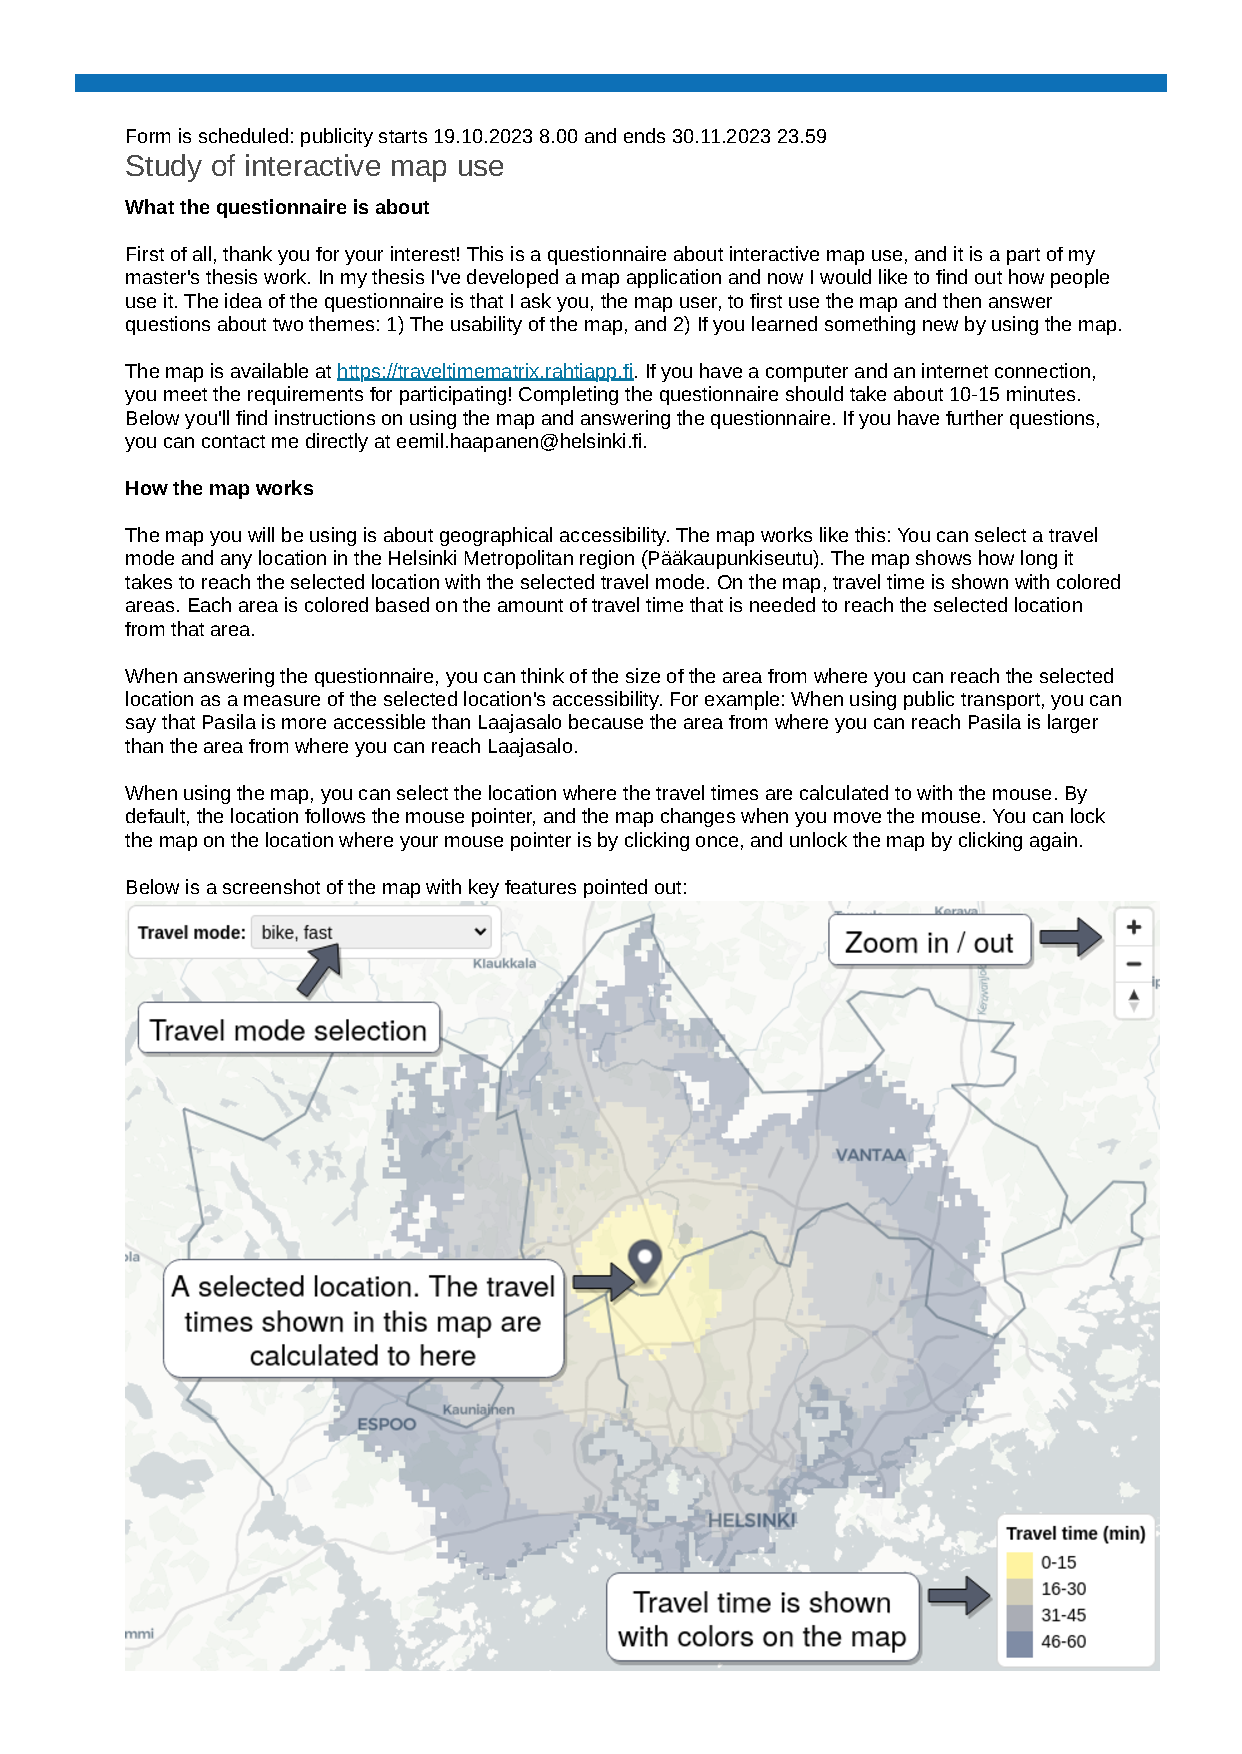
\includepdf[pages={1-},scale=0.9,pagecommand={}]{external_pdf/questionnaire.pdf}

\subsection{Questionnaire responses}
\label{appendix:questionnaire responses}

Responses to the questionnaire are presented here.
They are divided into the same task groupings that were used in the questionnaire.

\sffamily

\begin{minipage}{\textwidth}
\textbf{Task 1}

\begin{figure}[H]
	\begin{subfigure}[b]{0.5\textwidth}
		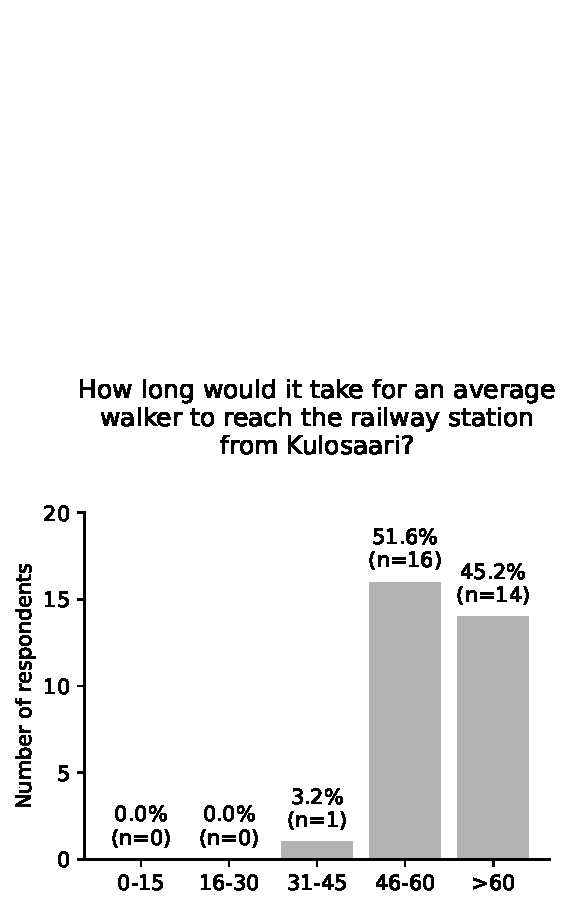
\includegraphics[width=\textwidth]{visual/figures/survey/0.pdf}
	\end{subfigure}%
	\hfill
	\begin{subfigure}[b]{0.5\textwidth}
		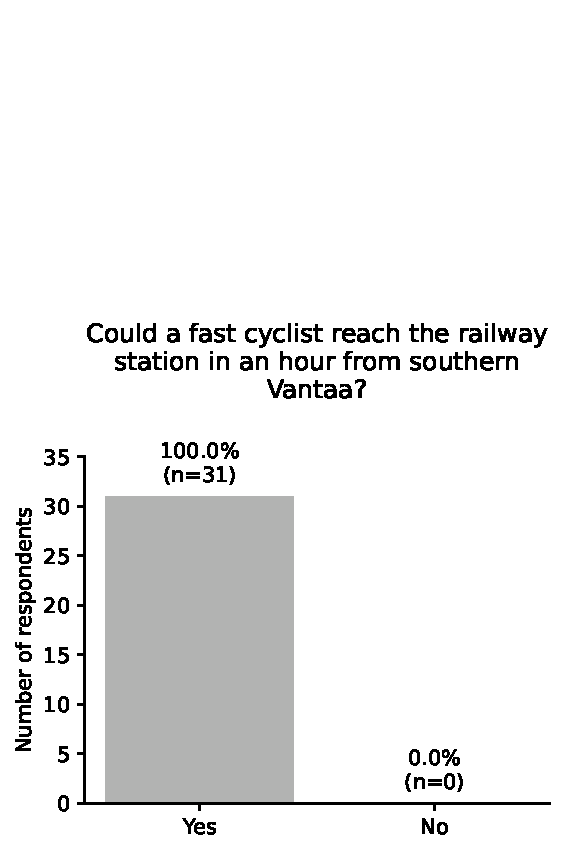
\includegraphics[width=\textwidth]{visual/figures/survey/1.pdf}
	\end{subfigure}%
\end{figure}
\end{minipage}

\begin{minipage}{\textwidth}
\textbf{Task 2}

\begin{figure}[H]
	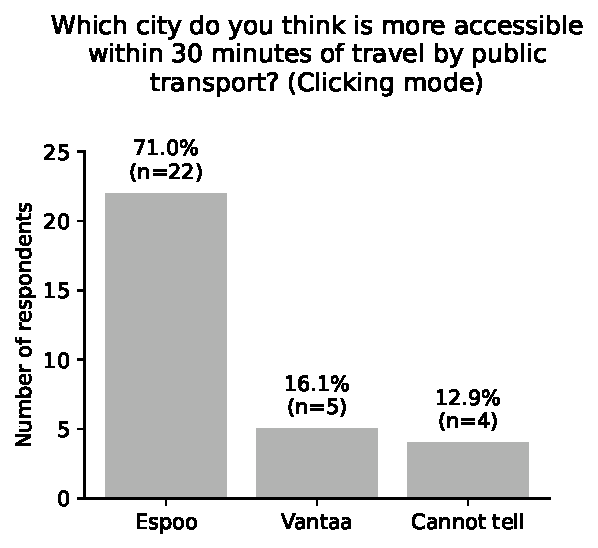
\includegraphics[width=0.5\textwidth]{visual/figures/survey/2.pdf}
\end{figure}
\end{minipage}

\begin{minipage}{\textwidth}
\textbf{Task 3}

\begin{figure}[H]
	\begin{subfigure}[b]{0.5\textwidth}
		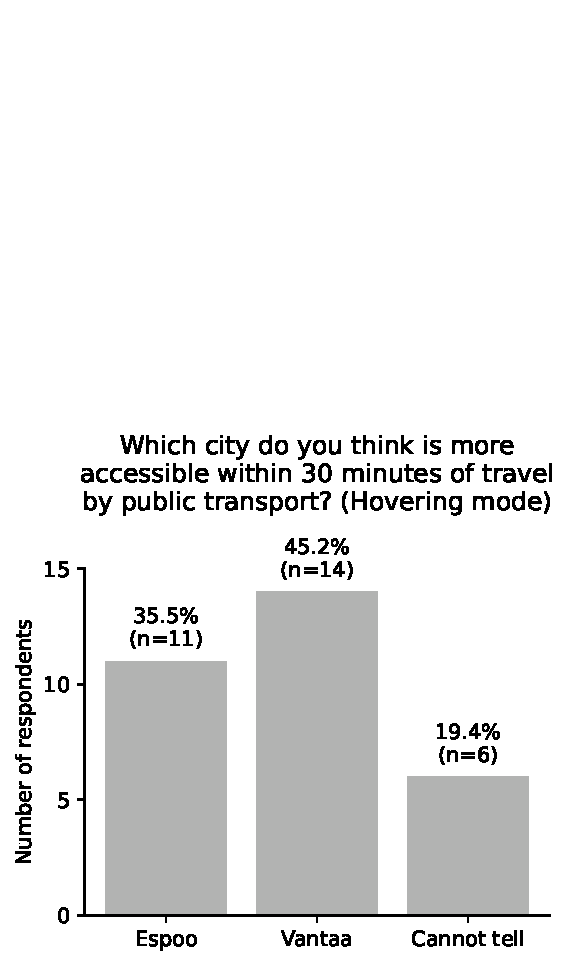
\includegraphics[width=\textwidth]{visual/figures/survey/3.pdf}
	\end{subfigure}%
	\hfill
	\begin{subfigure}[b]{0.5\textwidth}
		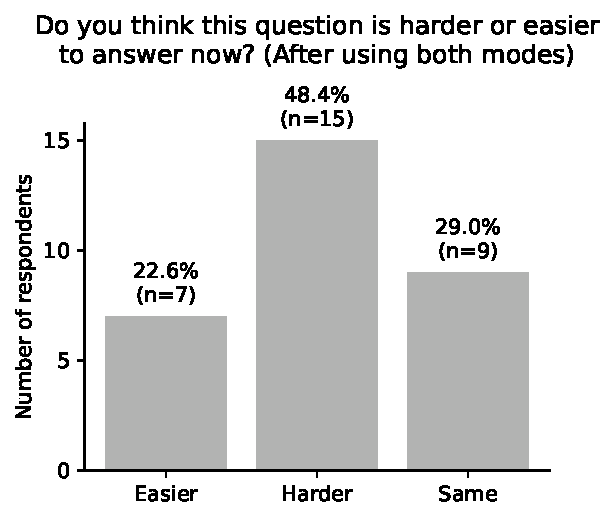
\includegraphics[width=\textwidth]{visual/figures/survey/4.pdf}
	\end{subfigure}%
\end{figure}
\end{minipage}

\begin{minipage}{\textwidth}
\textbf{Task 4}

\begin{figure}[H]
		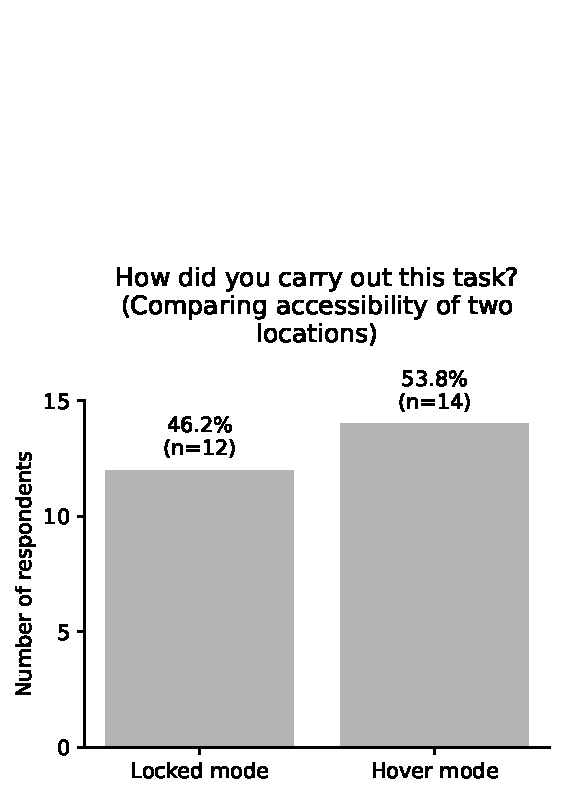
\includegraphics[width=0.5\textwidth]{visual/figures/survey/5.pdf}
\end{figure}
\end{minipage}

\begin{minipage}{\textwidth}
\textbf{Task 5}

\begin{figure}[H]
		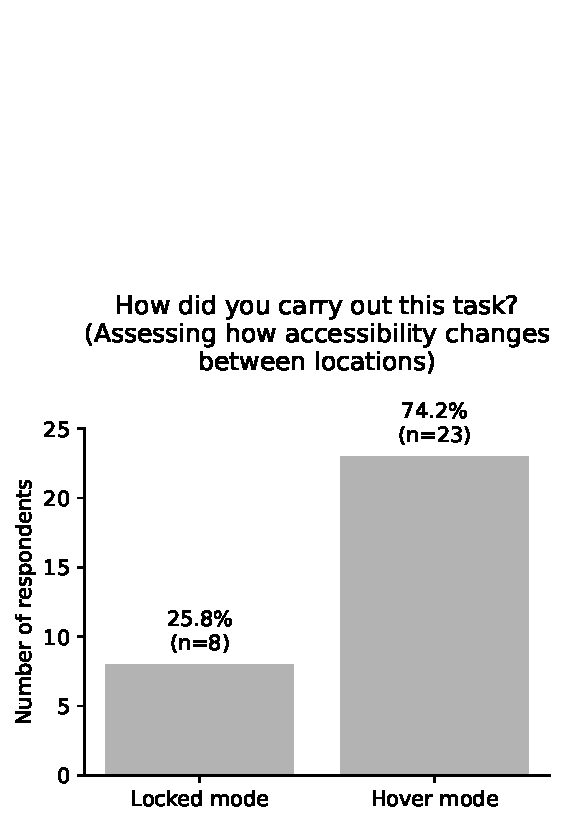
\includegraphics[width=0.5\textwidth]{visual/figures/survey/6.pdf}
\end{figure}
\end{minipage}

\begin{minipage}{\textwidth}
\textbf{General questions}

\begin{figure}[H]
	\begin{subfigure}[b]{0.5\textwidth}
		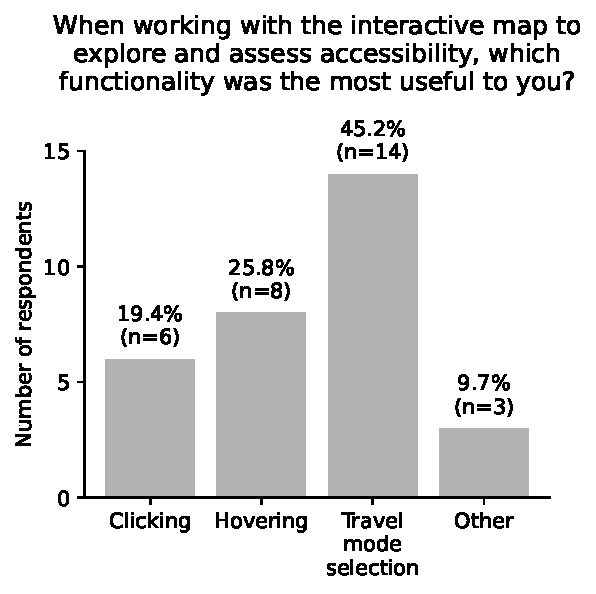
\includegraphics[width=\textwidth]{visual/figures/survey/7.pdf}
	\end{subfigure}%
	\hfill
	\begin{subfigure}[b]{0.5\textwidth}
		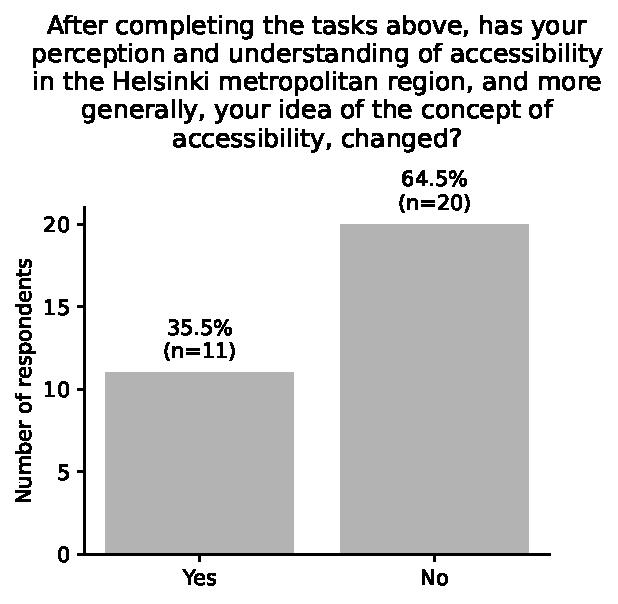
\includegraphics[width=\textwidth]{visual/figures/survey/8.pdf}
	\end{subfigure}%
	\newline
	\begin{subfigure}[b]{0.5\textwidth}
		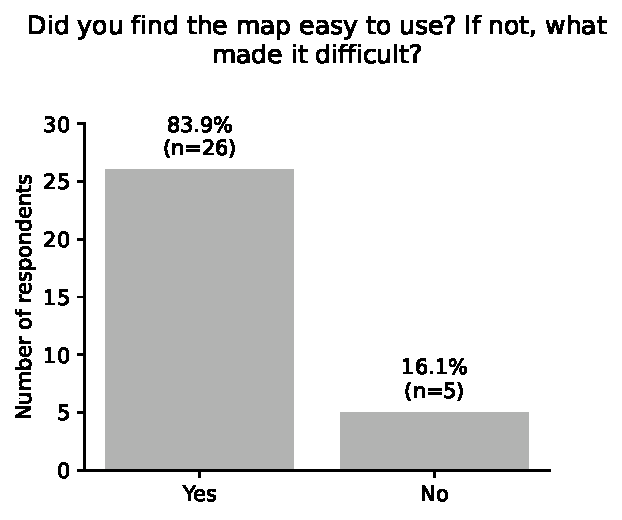
\includegraphics[width=\textwidth]{visual/figures/survey/9.pdf}
	\end{subfigure}%
\end{figure}
\end{minipage}

\begin{minipage}{\textwidth}
\textbf{Background information}

\begin{figure}[H]
	\begin{subfigure}[b]{0.5\textwidth}
		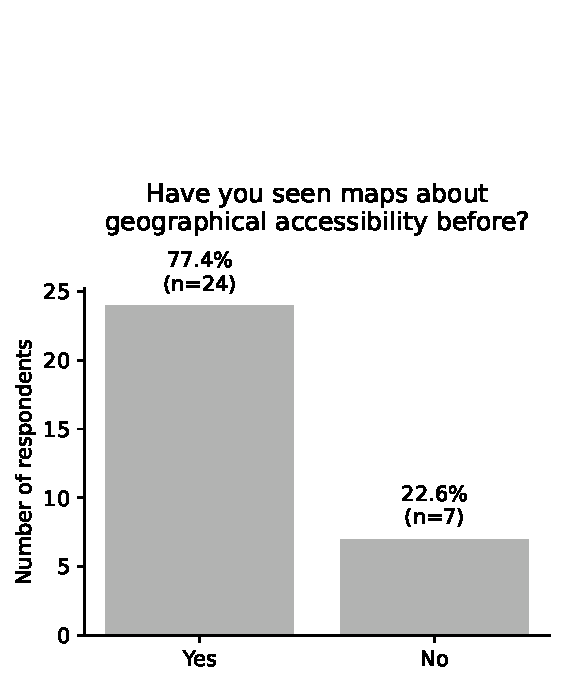
\includegraphics[width=\textwidth]{visual/figures/survey/10.pdf}
	\end{subfigure}%
	\hfill
	\begin{subfigure}[b]{0.5\textwidth}
		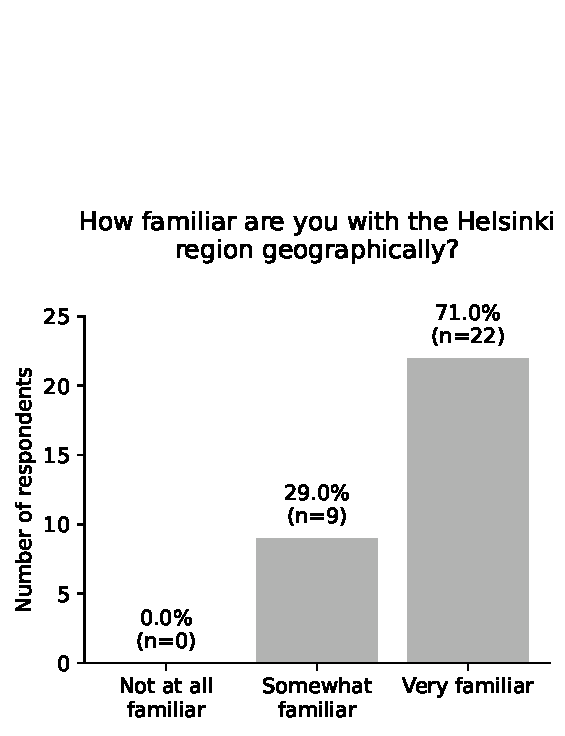
\includegraphics[width=\textwidth]{visual/figures/survey/11.pdf}
	\end{subfigure}%
	\newline
	\begin{subfigure}[b]{0.5\textwidth}  % [t] to position to top
		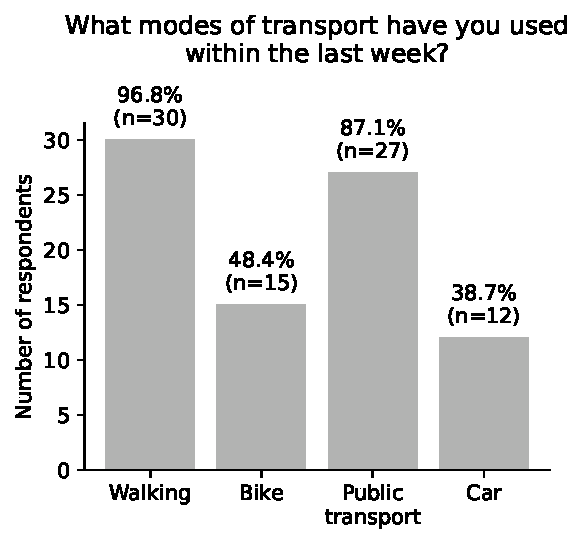
\includegraphics[width=\textwidth]{visual/figures/survey/modes.pdf}
	\end{subfigure}%
	\begin{subfigure}[b]{0.5\textwidth}
		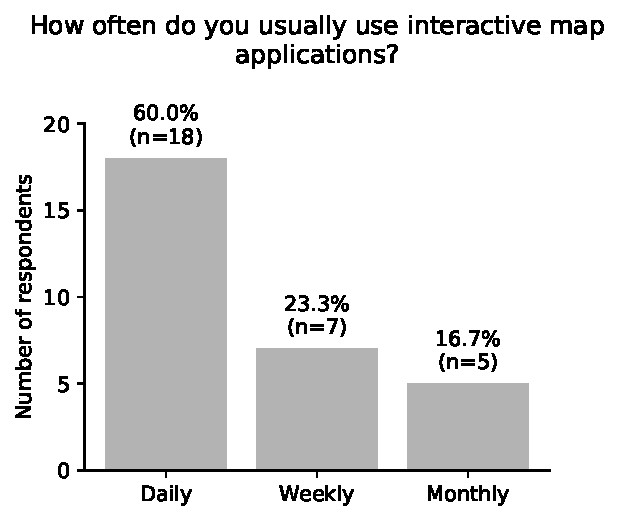
\includegraphics[width=\textwidth]{visual/figures/survey/12.pdf}
	\end{subfigure}%
\end{figure}
\end{minipage}

\begin{minipage}{\textwidth}
\textbf{Demographic information}

\begin{figure}[H]
	\begin{subfigure}[b]{0.5\textwidth}
		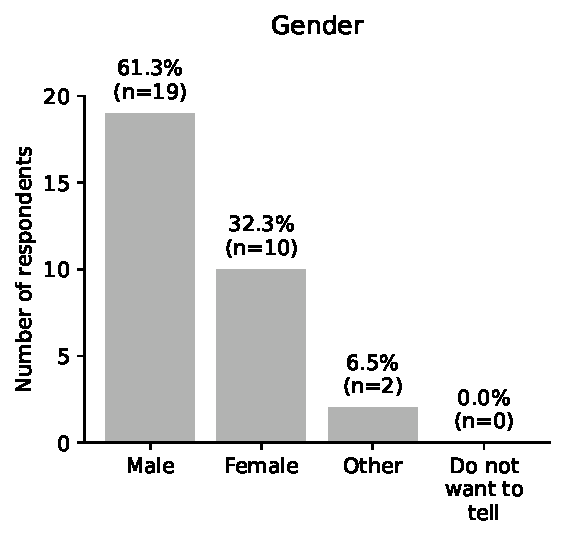
\includegraphics[width=\textwidth]{visual/figures/survey/13.pdf}
	\end{subfigure}%
	\hfill
	\begin{subfigure}[b]{0.5\textwidth}
		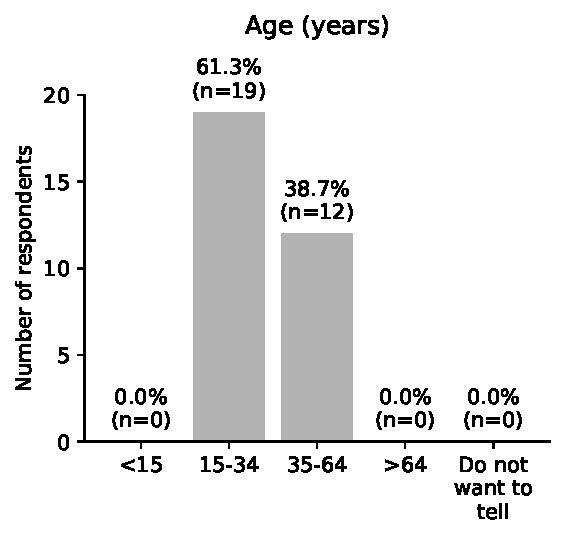
\includegraphics[width=\textwidth]{visual/figures/survey/14.pdf}
	\end{subfigure}%
\end{figure}
\end{minipage}

\end{appendices}
